
\chapter{Øyesporing}

I dette kapittelet blir det gitt enkel forklaring over øyet og hvordan der er mulig å spore det ved hjelp av en øyesporingsenhet. Til slutt vil enheten som brukes i prototype og hvordan den brukes bli presentert.


\section{Hvordan fungerer øyet?}

Å forklare hvordan øyet fungerer i detalj er utenfor denne rapportens omfang. Det vil derimot gitt en enkel forklaring av hvordan det fungerer og de mest nødvendige konseptene.

\subsection{Synsfelt}

I en artikkel skrevet av Tobii \cite{Calibration} sammenlignes øyet med et fotoapparat på grunn av dens mange likhetstrekk. Det hele starter ved at når lys treffer et objekt så reflekteres det. Og på samme måte som et kamera så fanges det reflekterte lyset opp av en linse, som igjen prosjekterer det på en lyssensitiv overflate. Men i motsetning til et kamera er ikke denne overflaten like sensitiv overalt i øyet. Dette gjør at menneske kan tilpasse synet etter hvor mye lys som er tilgjengelig. En bieffekt er at menneske kun kan se klart i begrensede områder av synsfeltet. Dette er illustrert i Figur \ref{fig:visueltArea}, som viser hvordan synsfeltet hos menneske er delt inn etter klarhet. Det innerste området notert ved bokstaven F representerer det foveale området, også kjent som skarpsynet. Dette er den delen av synsfeltet man fokuserer på og som man derfor oppfatter som klarest. Det er hovedsaklig fra dette området visuell data hentes fra. Området deklarert med bokstavene Pf i figuren viser det parafovela området. Som er et overgangsområde og kjennetegnes ved at uskarpheten gradvis øker til man kommer til det perifere området vist som P i figuren. Det perifere området, også kjent som sidesynet, er det mest uskarpe området og fungerer kun bra til å fange opp bevegelser og kontraster.

\begin{figure}[ht!]
\centering
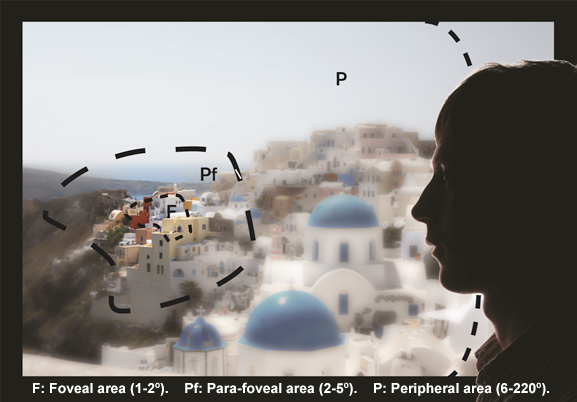
\includegraphics[width=65mm]{fovealArea}
\caption{Bilde/Illustrasjon av menneskelige synsfelt \cite{VisualImage}}
\label{fig:visueltArea}
\end{figure}

\subsection{Øyebevegelser}

Det foveale området er som tidligere nevnt det området det registreres mest visuell data. Ulempen er at området kun står for rundt 2 grader av synsfeltet \cite{Backg0:online}. Så hvis en ønsker å hente detaljert informasjon fra andre deler av synsfeltet, må det foveale området flyttes ved å bevege øyene. De ulike øyebevegelsene som brukes er beskrevet i Listen under er hentet fra nettsiden synstap \cite{sanse7:online}.

\subsubsection{Grovmotoriske}
\begin{itemize}
\item Akkomodasjon – øyets evne til å se klart på forskjellige avstander, det å kunne se skarpt når en flytter blikket hurtig fra avstand til nært og omvendt
\item Følgebevegelser – kunne følge en gjenstand med blikket i alle retninger uten å bevege hodet
\item Konvergens – kunne holde blikket samlet på nært hold
\item Stereosyn – evnen til å se avstand og dybde
\end{itemize}
\subsubsection{Finmotoriske}
\begin{itemize}
\item Sakkader – små forflytninger med blikket ved for eksempel lesing
\item Minisakkader – minibevegelser av øyet (dirring), som må være tilstede for at det skal sendes informasjon til hjernen
\item Antisakkader – evnen til å undertrykke en øyebevegelse
\item Fiksering – evnen til å holde blikket stødig festet på ett punkt
\end{itemize}



\section{Hva er øyesporing?}

Øyesporing er prosessen med å måle hvor en person ser, eller bevegelsen til et øye i forhold til hodet \cite{Eye t4:online}. Ved å gjøre dette kan man finne ut hvilke elementer brukeren ser på, hvor lenge han ser på det og hvordan han beveger blikket. 


\subsection{Bruksområder}

Øyesporing kan anvendes på flere måter. Blant annet så brukte Alfred L. Yarbus øyesporing det til forskning. I sin artikkel fra 1967 \cite{wexle4:online} beskriver han hvordan et subjekts øyebevegelser blir påvirket av oppgaven han skal gjennomføre. Bilde \ref{fig:yarbus} viser hvor forskjellig en person ser på et bilde basert på hvilken oppgave han er tildelt. I tilegg til vitenskap brukes øyesporing også til markedsundersøkelser, reklame, brukervennlighets-testing og mer \cite{Case2:online}. Det som kjennetegner de nevnte bruksområdene er at brukeren ikke aktivt foretar seg noe, han bruker ikke øyene til å gjøre noe annet enn å se. Noe som er annerledes fra anvendelsen i denne oppgaven, hvor øyene i tilegg til å se, brukes til interaksjon.



\begin{figure}[ht!]
\centering
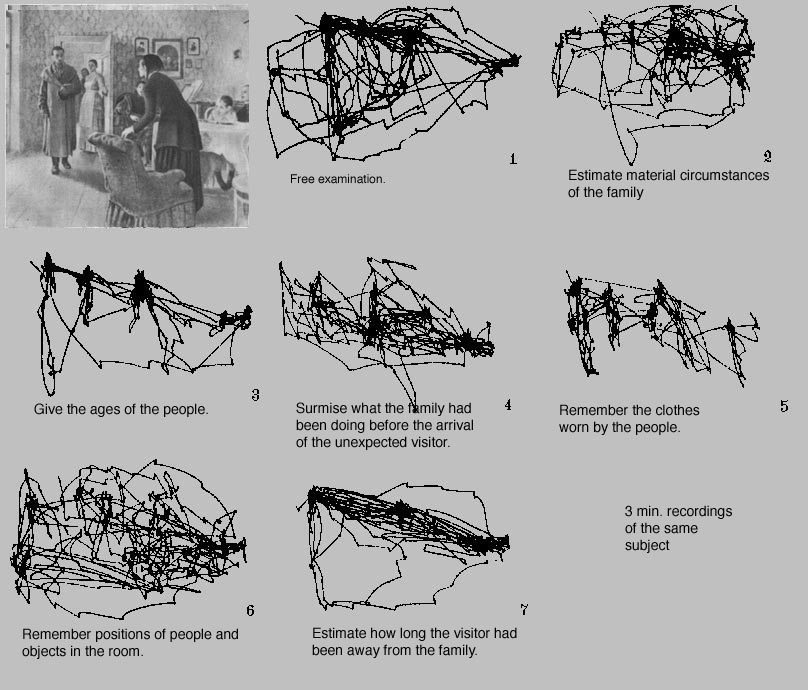
\includegraphics[width=100mm]{Yarbus_The_Visitor}
\caption{Bilde som viser hvordan et subjekts øyebevegelser påvirkes av oppgaven \cite{Yarbu2:online}}
\label{fig:yarbus}
\end{figure}


\subsection{Pupil Centre Cornea Reflection}

Øyesporing er som tidligere nevnt teknikken brukt til å fange og måle øyebevegelser. Det finnes derimot flere fremgangsmåter. I denne oppgaven vil det brukes en ikke-forstyrrende øyesporingsenhet. Dette gjør at brukeren i prinsippet ikke skal legge merke til enheten. For denne typen øyesporing er det mest vanlig å bruke en teknikk som heter Pupil Centre Cornea Reflection (\gls{PCCR}) \cite{Calibration}. Teknikken fungerer ved at en lyskilde belyser øyet for at refleksjonene skal bli klare og synlige. Et kamera tar deretter bilde av refleksjonene fra øyet. Bildet blir så brukt til å identifisere lysets refleksjon på hornhinnen og pupillen. Når en vet vinkelen mellom hornhinnen og pupillen er det mulig å regne ut en vektor. Vektoren sammen med andre geometriske egenskaper ved refleksjonene gjør det mulig å kalkulere ut blikkretningen(Der brukeren ser) \cite{Calibration}.


\section{Tobii PCEye Go}

I prototypen har vi valgt å ta i bruk øyesporingsenheten Tobii PCeye GO \cite{Contr4:online}, som er vist på bilde \ref{fig:tobiiPc}. Enheten kommer separat og kobles til datamaskinen via USB. Denne enheten ble valgt fordi den brukes i Sono Flex og fordi kontaktpersonen i Tobii allerede hadde god erfaring med enheten. Den har også den foredelen at den er av den ikke-forstyrrende typen. Det vil si at en bruker i teorien ikke vil plages av enheten. Noe som hadde vært tilfelle ved å bruke brillene vist på bilde \ref{fig:tobii_glasses} til øyesporing.


\begin{figure}[ht!]
\centering
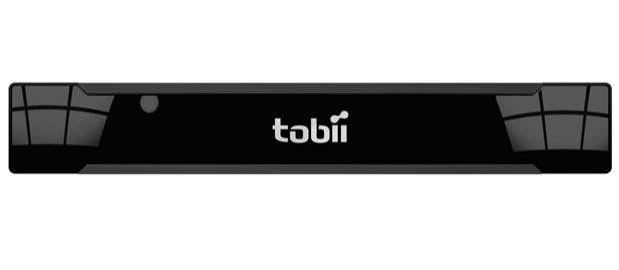
\includegraphics[width=50mm]{TobiiEyeGo}
\caption{Bilde av øyesporingsenheten Tobii PCEye Go}
\label{fig:tobiiPc}
\end{figure}

\begin{figure}[ht!]
\centering
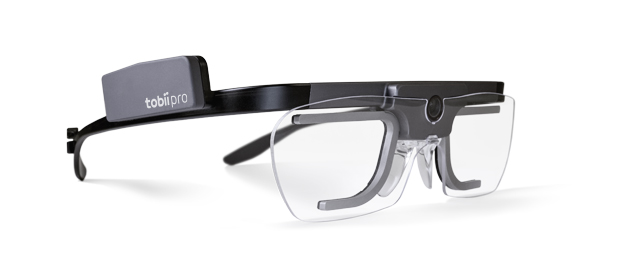
\includegraphics[width=50mm]{Tobii_Glasses}
\caption{Øyesporingsenhet i form av briller som brukeren har på seg}
\label{fig:tobii_glasses}
\end{figure}


\subsection{Tobii Eye Control API }

Figur \ref{fig:overview} viser hvordan blikk interaksjonsserveren eksponerer funksjonalitet til en klient-applikasjon gjennom APIet kalt Tec API. For å ta i bruk TecAPIet tilbys to aksess punkter. Et gjennom .NET plattformen kalt TecClient og et for C dynamisk link library kalt MPACI.  Den praktiske betydningen, er at man kun kan bruke APIet ved å skrive i C eller .NET teknologier. I denne rapporten vil kun sistnevnte være interessant, altså .NET APIet kalt TecClient.


\begin{figure}[ht!]
\centering
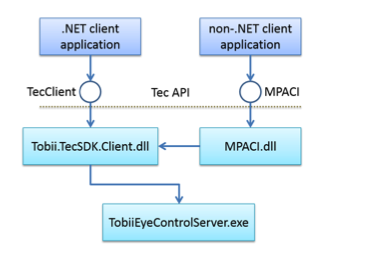
\includegraphics[width=100mm]{SoftwareArchitectureOverview}
\caption{Bilde som viser programvare arkitekturen til blikk programvaren}
\label{fig:overview}
\end{figure}


\subsection{TecClient}

For å gi tilgang til API funksjoner er TecClient komponentet for .NET delt inn i verktøys klasses(toolbox classes). Figur \ref{fig:toolbox} viser de ulike verktøyene som er tilgjengelig. 

\begin{figure}[ht!]
\centering
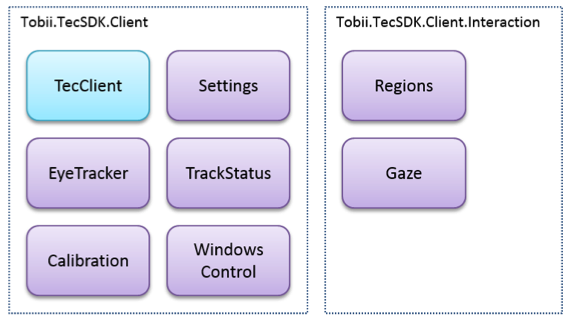
\includegraphics[width=100mm]{Toolbox}
\caption{Verktøy klassser som er tilgjengelige gjennom TecClient komponenten verktøyskasse}
\label{fig:toolbox}
\end{figure}


\textbf{EyeTracker} Gir informasjon om den aktuelle øyesporingsenheten. 

\textbf{Kalibrering} 
For optimal øyesporing med Tobii PCeye Go må enheten kalibreres for hver bruker. Dette verktøyet går gjennom en prosedyre for å måle karakteristikk ved personens øyer som brukes igjen til å lage en fysiologisk 3d modell for å kalkulere hvor brukeren ser \cite{www.t5:online}. Bilde \ref{fig:kalibre} viser et bilde fra kalibreringsprosessen, hvor brukeren blir bedt om å se på de ulike punktene.

\begin{figure}[ht!]
\centering
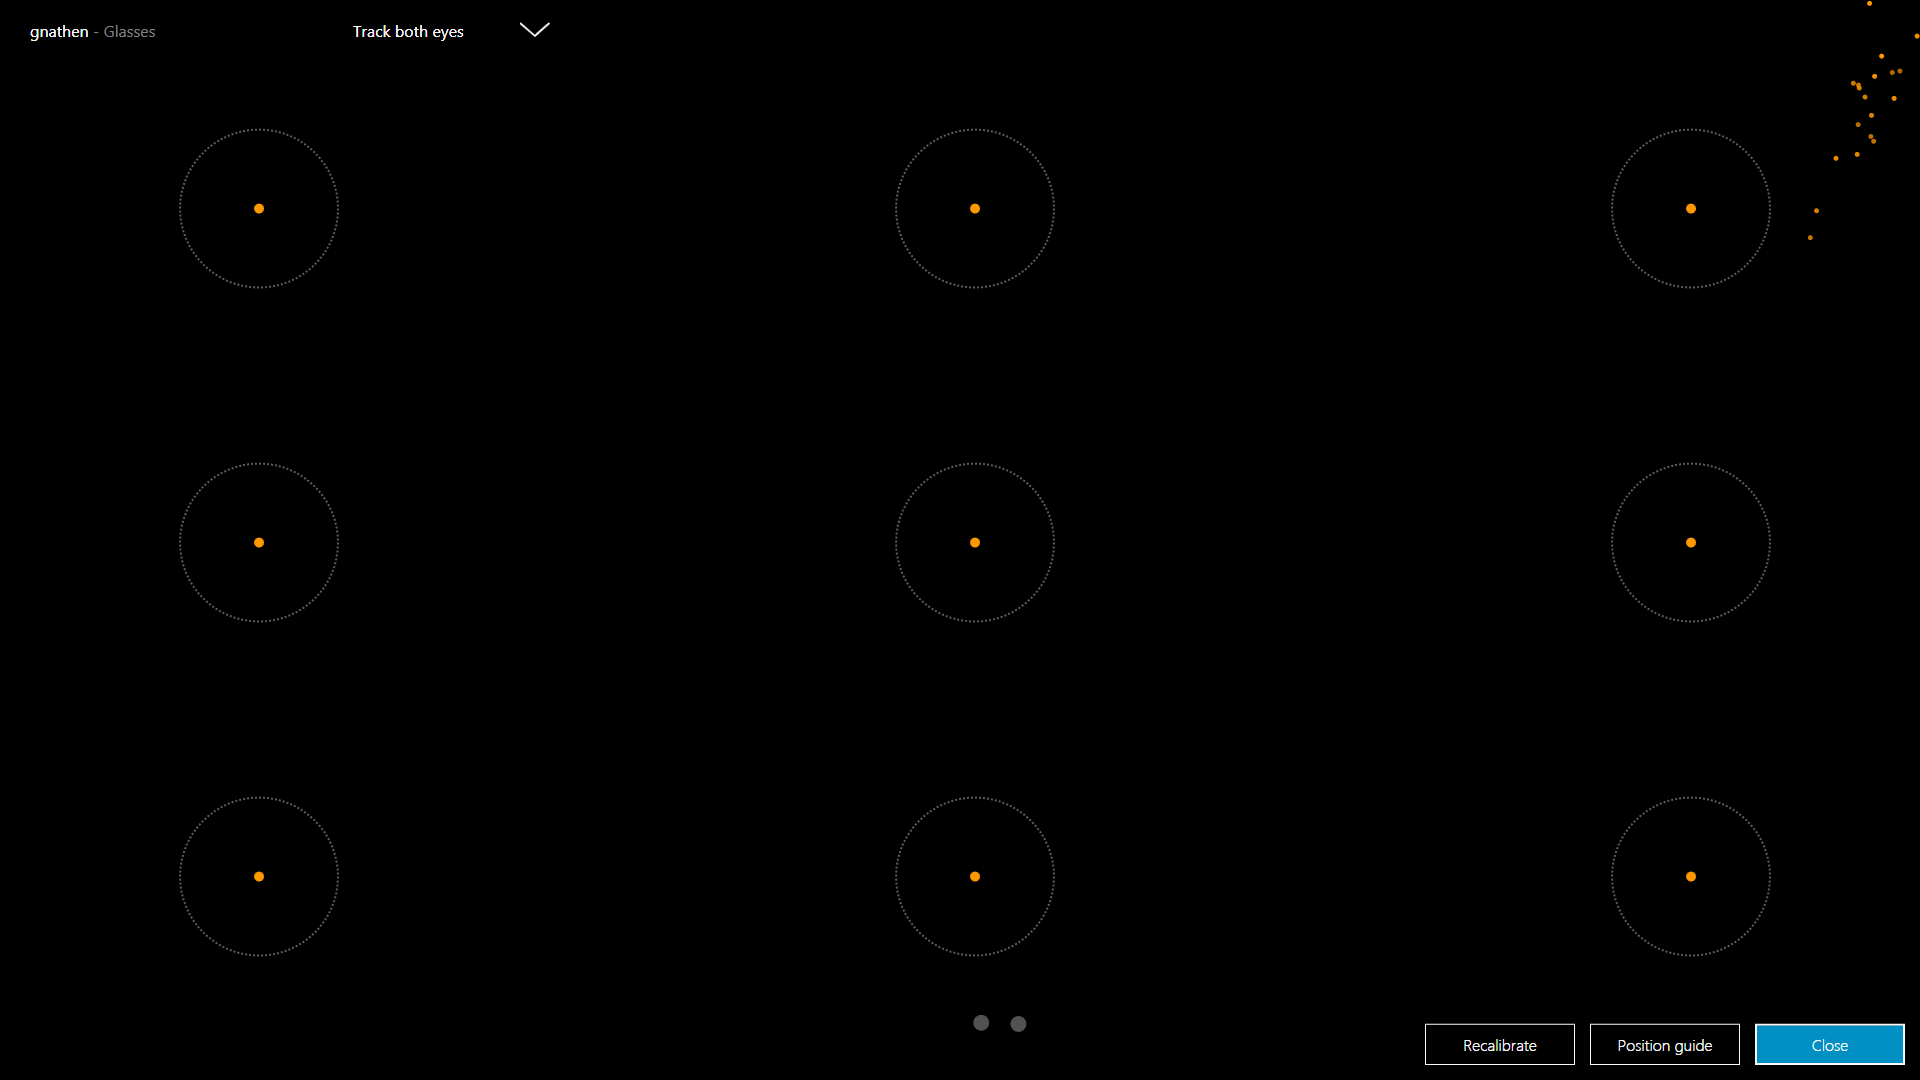
\includegraphics[width=100mm]{kalibrering}
\caption{ \cite{VHye88:online}}
\label{fig:kalibre}
\end{figure}


\subsubsection{Settings}
Settings komponente gir tilgang til brukerprofiler og operasjoner som gjør at man kan skifte mellom dem. For eksempel er det naturlig at en bruker ikke vil gå gjennom kalibreringsprosessen hver gang han vil ta i bruk enheten. I dette komponentet kan karakteristikken fra kalibreringen lagres i brukerprofilen som er er koblet til brukeren, slik at han slipper dette. 


\subsubsection{Trackstatus}
Tilbyr metoder, egenskaper og hendelser for å kontrollere sporingsstatus vinduet. Bilde \ref{fig:track} viser hvordan dette komponentet kan brukes til å vise brukeren om enheten fanger opp øyene og hvordan de er iforhold.

\begin{figure}[ht!]
\centering
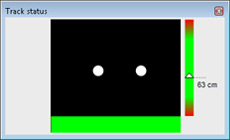
\includegraphics[width=100mm]{Trackstatus}
\caption{}
\label{fig:track}
\end{figure}

\subsubsection{Gaze}
Eksponerer rå blikkdata, både filtrert og ufiltrert. Det vil si at man kan kan finne ut hvor på skjermen en bruker ser i form av X og Y koordinater.


\subsubsection{Region / Interaction regions}

Ifølge dokumentasjonen er en interaksjon region er en geometrisk region på skjermen som en bruker kan interagere ved å se på den (dokumentasjon). En knapp i applikasjon vil typisk bli definert som en interaksjon region. Ved å definere en region kan man lytte til hendelser fra dem. De to viktigste hendelsene er \textbf{Focus} og \textbf{Activation}. Focus hendelsen vil aktiveres når en bruker skuer innenfor grensene til en region. En bruker vil bli opplyst om at han er innenfor en slik region ved hjelp av en indikator. Denne indikatoren vil typisk gi brukeren et signal om at en nedtelling har startet. Når nedtelling er ferdig vil Activation hendelsen bli avfyrt. Activation er konseptuelt det samme som å klikke med en datamus, og responsen vil normalt være den samme.




